\documentclass[a4paper]{article}

\usepackage[T5]{fontenc}
\usepackage[utf8]{inputenc}
\usepackage{amsfonts}
\usepackage{mathtools}
\usepackage[iso]{datetime}
\usepackage{tabu}
\usepackage[colorlinks=true,urlcolor=blue,linkcolor=black]{hyperref}
\usepackage{listings}
\usepackage{tikz}

\usetikzlibrary{shapes.geometric}
\tikzset{
  treenode/.style = {align=center, inner sep=0pt, text centered, font=\sffamily},
  tnode/.style = {treenode, circle, black, solid, draw=black, inner sep=2pt, minimum width=1.5em},
  subtree/.style = {draw,dashed,shape border uses incircle, isosceles triangle,shape border rotate=90, minimum height=0.5cm},
  tnull/.style = {treenode, rectangle, draw=black, minimum width=0.5em, minimum height=0.5em},
  level/.style = {sibling distance=2cm, level distance=1cm},
}

\title{Advanced Data Structures\\\large Lecture 10}
\date{2017-01-12 \\ Last edited \currenttime\ \today}
\author{Lecture by Dr. Shay Mozes\\Typeset by Steven Karas}

\newenvironment{itemize*}%
  {\begin{itemize}%
    \setlength{\itemsep}{0pt}%
    \setlength{\parsep}{0pt}%
    \setlength{\parskip}{0pt}}%
  {\end{itemize}}

\newenvironment{enumerate*}%
  {\begin{enumerate}%
    \setlength{\itemsep}{0.5pt}%
    \setlength{\parsep}{0pt}%
    \setlength{\parskip}{0pt}}%
  {\end{enumerate}}

\begin{document}

\maketitle

\section{Review of Dynamic trees}

For this represented tree:

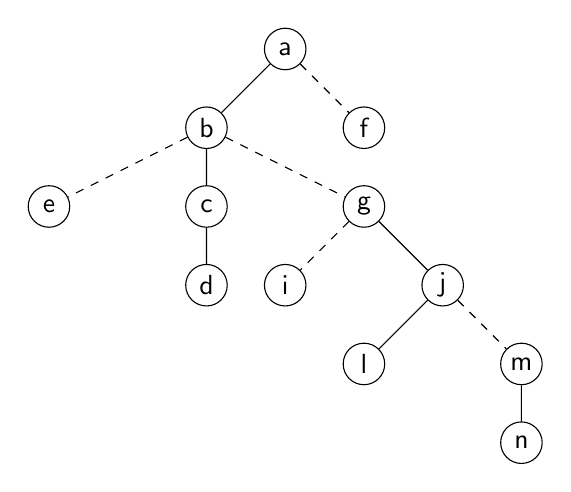
\begin{tikzpicture}
\node [tnode] (P) {a}
  child{ node [tnode] {b}
    child[dashed]{ node [tnode] {e} }
    child{ node [tnode] {c}
      child{ node [tnode] {d} }
    }
    child[dashed]{ node [tnode] {g}
      % NOTE: h was deleted because it just got in the way
      child[dashed]{ node [tnode] {i} }
      child[solid]{ node [tnode] {j}
        child[solid]{ node [tnode] {l} }
        child[dashed]{ node [tnode] {m}
          child[solid]{ node [tnode] {n} }
        }
      }
    }
  }
  child[dashed]{ node [tnode] {f} }
;
\end{tikzpicture}

We get a concrete forest of splay trees:

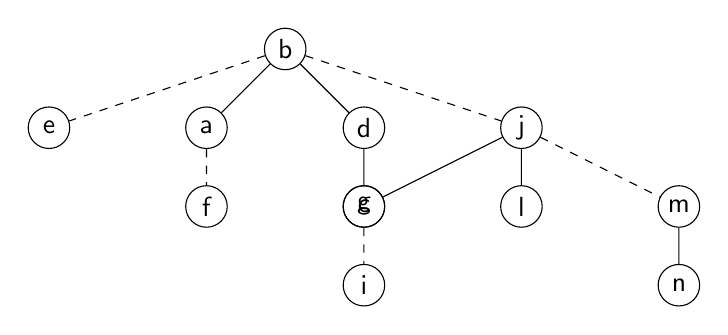
\begin{tikzpicture}
%TODO: figure out how to draw the surrounding subtrees
%TODO: figure out how to fix the overlapping nodes
\node [tnode] (P) {b}
  child[dashed]{ node [tnode] {e}}
  child[solid]{ node [tnode] {a}
    child[dashed]{ node [tnode] {f} }
  }
  child[solid]{ node [tnode] {d}
    child[solid]{ node [tnode] {c}}
  }
  child[dashed]{ node [tnode] {j}
    child[solid]{ node [tnode] {g}
      child[dashed]{ node [tnode] {i}}
    }
    child[solid]{ node [tnode] {l}}
    child[dashed]{ node [tnode] {m}
      child[solid]{ node [tnode] {n}}
    }
  }
;
\end{tikzpicture}

\subsection{Topological operations}

\subsubsection{MakeTree\texorpdfstring{$(v)$}{(v)}}
Create a tree with a single node $v$.

\subsubsection{FindRoot\texorpdfstring{$(v)$}{(v)}}
Returns the root of the tree that contains $v$.

\subsubsection{Cut\texorpdfstring{$(v)$}{(v)}}
Assume that $v$ is not a root. Deletes the edge from $v$ to its parent.

\subsubsection{Link\texorpdfstring{$(v,w)$}{(v,w)}}
Given two nodes $v,w$.
Assume that $v$ is the root of its tree, and $v,w$ are not in the same tree.
Attach the tree of $v$ as a child of $w$.

\subsubsection{Expose\texorpdfstring{$(v)$}{(v)}}
This is the difficult primitive that will help us implement all the other operations efficiently. This operation makes the path from $v$ to the root a favored path and marking all favored edges that are incident to the path to unfavored. It has the side effect of making $v$ the root of the concrete tree.

\begin{lstlisting}[frame=L]
Expose(v):
  Splay(v)
  v.right = nil
  while v.parent != nil:
    w = v.parent
    Splay(w)
    w.right = v
    rotateUp(v)
\end{lstlisting}

$\underbrace{O(\log n)}_{\text{Splay}} \cdot \underbrace{\text{\# changes of favored children}}_{\text{\# iterations of the loop}}$

\subparagraph{Lemma}
The number of changes of favored children in a sequence of $m$ operations is $O(n + m \log n)$

A full proof including a heavy-light decomposition was in the previous lecture.

We have shown a bound of $O((n+m\log n) \log n)$ on a sequence of $m$ operations.

In a sequence of $m$ operations, we get a bound of: $O(n\log n + m \log^2 n)$ that gives us an amortized cost of $O(\log^2 n)$.

\paragraph{Reminder: Splay tree complexity}
Each node $v$ has a weight $w(v)$. Let $S(x)=\sum_{\text{$u$ descendent of $v$}} w(u)$.
Let $\phi_{splay}(T)=\sum_{v \in T} \log(S(v)$.
$amort(splay\ v) \le 3(\log S(root) - \log S(v))$

\paragraph{Amortized complexity using potential function}
Define $S'(v)=$ the number of nodes in the subtree of $v$ in the concrete tree.
\[\phi_{LC}= \sum_{v \in T_\text{c}} \log S'(v)\]

Changing the favored child does not change the potential function.
Therefore the contribution of changing the favored child to the amortized cost of Expose is the number of changes: $O(n+m\log n)$.

\paragraph{Changes of Splay to the potential function}
Let $w'(v)=1+\sum_{u\text{ unfavored children of }v} \; S'(u)$.

For example, in our example above, $S'(j)=5$, yet $w'(v)=2$.

Therefore: $S(v)= \sum w'(u) = S'(v)$

The contribution of each splay operation to the amortized cost is $\le 3(\log S(root_{splay}) - \log S(v))$.
Because the node $v_{i+1}$ that is splayed in the $i+1$ step is the parent of the $root_i$ in the $i^{\text{th}}$ iteration $S(v_{i+1}) \ge S(root_i)$, the series is telescopic.

Therefore the contribution of each splay of an Expose$(v)$ is at most $\log S'(root) - \log S'(v) = O(\log n)$.

Thus the total cost of a sequence of $m$ operations is:
\[O(n+m\log n)+O(m\cdot \log n) = O(n+m\log n)\]

\subsection{Decorative Operations}
Instead of storing the cost of each node from the represented tree, we store the $\Delta$:

\[
\Delta c(v)=\begin{cases}
c(v) & v\text{ is a root} \\
c(v) - c(parent(v)) & \text{else}
\end{cases}
\]

Which gives us that $c(u)=\Delta c(u)$ if $u$ is a root, and $c(u)=\Delta c(u) + c(v)$ if $u$ is a child of $v$.

This guarantees us that for any node $u$, $c(u)=\sum_{v\text{ ancestor of }u}\Delta c(v)$.
\footnote{We will prove in the homework that the rotation updates the costs correctly}

\paragraph{Example with $c(v)$/$\Delta c(v)$:}\ \\
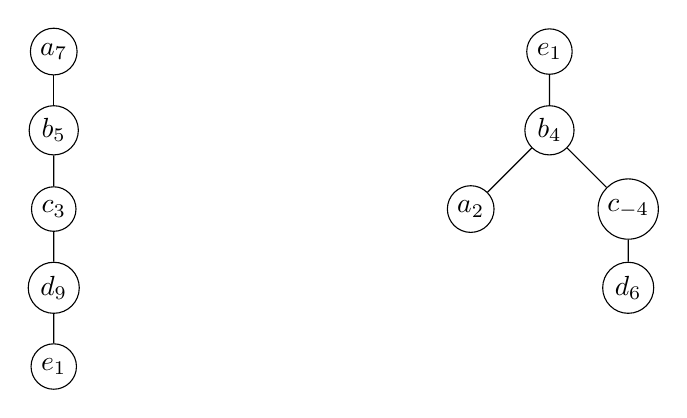
\begin{tikzpicture}
\node [tnode] (P) {$a_7$}
  child[solid]{ node [tnode] {$b_5$}
    child[solid]{ node [tnode] {$c_3$}
      child[solid]{ node [tnode] {$d_9$}
        child[solid]{ node [tnode] {$e_1$} }
      }
    }
  }
;

\node [tnode, right of=P, right=5cm] (S) {$e_1$}
  child[solid]{ node [tnode] {$b_4$}
    child[solid]{ node [tnode] {$a_2$} }
    child[solid]{ node [tnode] {$c_{-4}$}
      child[solid]{ node [tnode] {$d_{6}$}}
    }
  }
;
\end{tikzpicture}

\subsubsection{AddCost\texorpdfstring{$(v, x)$}{(v, x)}}
Add $x$ to the weight of each node on the path from $v$ to the root.

\begin{lstlisting}[frame=L, mathescape=true]
AddCost(v, x):
  Expose(v)
  v.$\Delta$c += x
\end{lstlisting}

\subsubsection{FindMinCost\texorpdfstring{$(v)$}{(v)}}
Find the first node with minimal cost on the path from $v$ to the root.

Define the following:
Let $\min c(v)=$ the minimal $c(v)$ in the subtree of the concrete splay tree of $v$.

\[\Delta c(v)=c(v)-\min c(v)\]
\[
\Delta \min c(v)=\begin{cases}
  \min c(v) & \text{$v$ is a root}\\
  \min c(v) - \min c(parent(v)) & \text{else}
\end{cases}
\]

\[\min c(u)=\sum_{v\text{ ancestor of }u}\Delta \min c(v)\]
\[c(u)=\Delta c(u) + \min c(u)\]

\begin{lstlisting}[frame=L, mathescape=true]
FindMinCost(v):
  Expose(v)
  Repeat:
    if v.left.$\Delta$minc=0:
      v = v.left
    else if $\Delta$c(v) > 0:
      v = v.right
    else:
      break
  Splay(v)
  return v
\end{lstlisting}

\subsubsection{Evert}
\footnote{There was a hint that this may appear in the next homework}

\paragraph{History}
In the original presentation of Link-Cut trees, splay trees were not yet discovered (or rather, were being discovered in parallel). As a result, the original complexity was much worse, and only after they combined them the complexity went down.

\section{Euler tour trees}
These trees are used to solve the problem of dynamic connectivity in graphs.
For simplicity, we will assume that our link-cut trees are rooted, and the root does not change.

\paragraph{History}
\href{http://dl.acm.org/citation.cfm?id=320215}{King and Henzinger 1999}


Note that the euler tour of the edges within this tree appear as such:

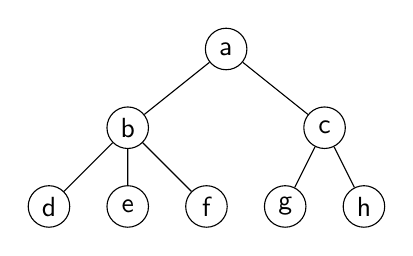
\begin{tikzpicture}
\node [tnode] (P) {a}
  child[sibling distance=2.5cm]{ node [tnode] {b}
    child[sibling distance=1cm]{ node [tnode] {d} }
    child[sibling distance=1cm]{ node [tnode] {e} }
    child[sibling distance=1cm]{ node [tnode] {f} }
  }
  child[sibling distance=2.5cm]{ node [tnode] {c}
    child[sibling distance=1cm]{ node [tnode] {g} }
    child[sibling distance=1cm]{ node [tnode] {h} }
  }
;
\end{tikzpicture}

\[\text{a}\underbrace{\text{bdbebfb}}_{\text{euler tour of subtree of b}}\text{acgchca}\]

So we build the binary search tree of the euler tour:

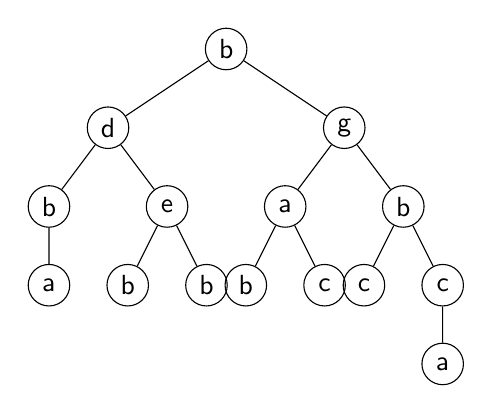
\begin{tikzpicture}
\node [tnode] (P) {b}
  child[sibling distance=3cm]{ node [tnode] {d}
    child[sibling distance=1.5cm]{ node [tnode] {b}
      child{ node [tnode] {a} }
    }
    child[sibling distance=1.5cm]{ node [tnode] {e}
      child[sibling distance=1cm]{ node [tnode] {b} }
      child[sibling distance=1cm]{ node [tnode] {b} }
    }
  }
  child[sibling distance=3cm]{ node [tnode] {g}
    child[sibling distance=1.5cm]{ node [tnode] {a}
      child[sibling distance=1cm]{ node [tnode] {b} }
      child[sibling distance=1cm]{ node [tnode] {c} }
    }
    child[sibling distance=1.5cm]{ node [tnode] {b}
      child[sibling distance=1cm]{ node [tnode] {c} }
      child[sibling distance=1cm]{ node [tnode] {c}
        child{ node [tnode] {a} }
      }
    }
  }
;
\end{tikzpicture}

Each edge points to both its nodes in the BST.
Each node points to some instance of itself in the BST.
Some implementations add an extra $k$ sentry node at the root.

\subsection{FindRoot}
Simply return the minimum in the BST.

\subsection{DeleteEdge}
Split and join around interval that is being removed.

\subsection{Reroot}
Rotate the euler tour to make the splice point the root (with cosmetic changes).

\subsection{AddEdge}
Reroot both trees and $O(1)$ splits and joins.

All of these are $O(\log n)$.

\end{document}
